\section{Retour d'expérience sur le Xeon Phi}
Le Xeon Phi est un co-processeur conçut par Intel.
%
Il s'agît d'une carte branchée en PCI express et qui permet de faire du calcul déporté.
%
Ce co-processeur est composé de 60 coeurs de calcul généralistes.
%
Ses coeurs de calcul supportent le jeu d'instructions x86 et ont la particularité de pouvoir maintenir 4 contextes simultanément.
%
Il s'agit de la technologie HyperThreading ou SMT\footnote{Simultaneous Multi Threading}.
%
Un changement de contexte est effectuer à chaque cycle.
%
L'utilisation de plusieurs threads par coeur à l'avantage de pouvoir masquer les temps d'attentes mémoire.
%
En parlant de mémoire, celle du Xeon Phi est en anneau et utilise l'interconnect (Fig.~\ref{fig:interconnect}).

%   (-_-)   %
\begin{figure}[t!]
  \centering
  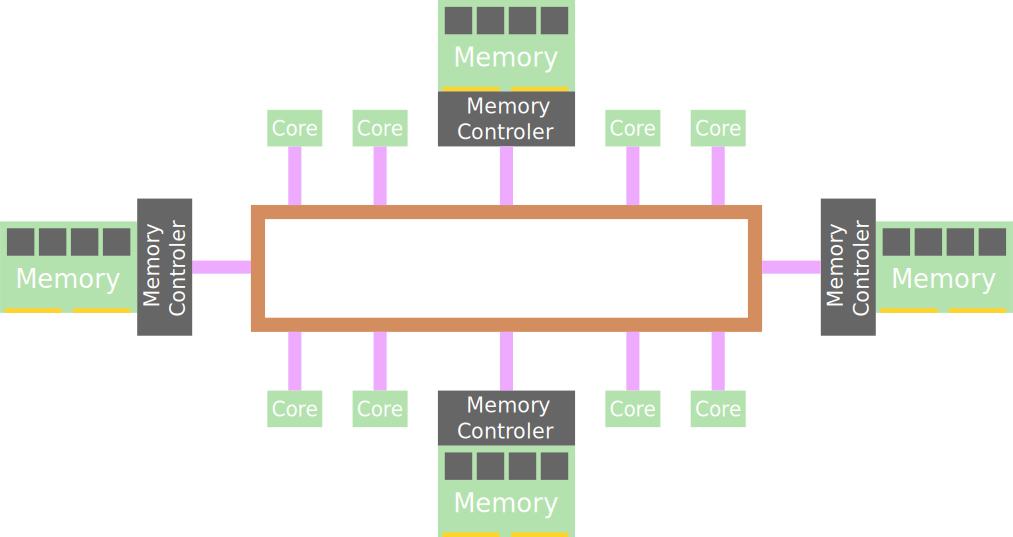
\includegraphics[width=\textwidth]{interconnect}
  \caption{Architecture en anneau du Xeon Phi.}
  \label{fig:interconnect}
\end{figure}


Nous avons de très bon débit mémoire comparé à un CPU classique.
%
Pour cette raison, il peut être intéressant de tester le produit matrice vecteur creux.
%
L'accélération maximale est de 120 par rapport à un coeur du Xeon Phi.
%
Mais il faut rappeler que ces coeurs ne sont pas faits pour exécuter du code séquentiel.
%
Les instructions sont exécutées dans l'ordre (in-order) et il n'y a donc pas de parallélisme d'instructions.
%
De plus, la fréquence d'horloge est basse (1,2~GHz) et le thread est exécuté un cycle sur 2 (600~MHz).
%
Il est donc très simple d'obtenir une bonne accélération par rapport à un coeur du Xeon Phi.
%
Par contre, si nous comparons l'accélération obtenue par rapport à un noeud de calcul, nous n'obtenons plus qu'une accélération de 2.
%
Ce qui est déjà bien mais pas suffisant pour espérer utiliser des Xeon Phi.
%
En effet, il y a deux modes de programmation dans le Xeon Phi :
\begin{itemize}
    \item le mode natif, qui consiste à faire tourner un noyaux Linux et à l'utiliser comme un noeud de calcul;
    \item le mode déporté, qui consiste à l'utiliser comme un accélérateur, à la manière d'un GPU.
\end{itemize}

Dans le mode natif, le code du simulateur de réservoir doit aussi tourner sur le Xeon Phi.
%
Or les parties séquentielles du code s'exécutent 10 fois moins vite que sur un CPU classique.
%
Donc les accélérations que nous obtenons sur les noyaux de calcul parallèle seront perdues à cause des parties séquentielle du code.


Le mode déporté ne fait pas mieux, pour pouvoir exécuter les noyaux de calcul sur le Xeon Phi, nous devons d'abord transférer les données qui seront utilisées.
%
Or, ce transfert coûtent du temps et ce temps cumulé à l'exécution du noyau de calcul est plus long que l'exécution du code sur le CPU.
%
De plus, ce mode ajoute de la complexité dans le code avec le support des transferts mémoires.
%
Cette complexité peut bien entendu être masqué par un runtime à base de tâches qui s'occupera des transferts mémoire à notre place.
